\chapter{Load Testing}

The purpose of load testing is to determine the ability of the application to perform during the key performance scenarios that we outlined in section 1.3. 


\section{Measurements}
In order to evaluate the ability of the application to meet its target we must use monitors that can measure the applications response time. As the HTTP responses do not contain client-side scripts or CSS we can measure response time as time to last byte (TTLB) of the HTML page. As well as measuring the average TTLB we must also measure the percentage of responses that are within the SLA as a large standard deviation may hide an unexpected number of failures within the average TTLB.

\section{Test Setup}
In order to simulate the expected user load we created a test using four different transactions. The transactions vary by the use of HTTP 1.0 and HTTP 1.1 with keep-alive TCP connections and the length of the "Think Time" between requests.

\begin{center}
\begin{tabular}{|l | c | c | c | c |}
\hline
ID & Weight & Think Time & HTTP & Keep-alive \\
\hline
1 & 10 & 300 & 1.0 & No \\ 
2 & 10 & 400 & 1.0 & No \\ 
3 & 40 & 300 & 1.1 & Yes \\ 
4 & 40 & 400 & 1.1 & Yes \\
    \hline
\end{tabular}
\end{center}

Microsoft's Web Capacity Analysis Tool (WCAT) was used as the primary testing software. The results where verified with a number of spot checks using JMeter. 

\begin{center}
\begin{tabular}{| c | c | c | c |}
\hline
Virtual Clients & Ramp up & Duration & Cool Down \\
\hline
150 & 300 & 600 & 60 \\ 
500 & 300 & 600 & 60 \\ 
1000 & 300 & 600 & 60 \\ 
\hline
\end{tabular}
\end{center}

Before each test the Jboss server is restarted and a warm-up test was is carried out with the following settings. 
\begin{center}
\begin{tabular}{| c | c | c | c |}
\hline
Virtual Clients & Ramp up & Duration & Cool Down \\
\hline
20 & 40 & 300 & 20 \\ 
\hline
\end{tabular}
\end{center}

\section{Results}
We carried out load testing in order to get a baseline of system performance in regard to our key performance scenarios. We looked at both client-side and server-side measures. 
\subsection*{Throughput} 
The throughput for the overall test is measured to determine the number of transactions the application can complete within each given time.

\begin{figure}[h]
\centering
\scalebox{0.65}{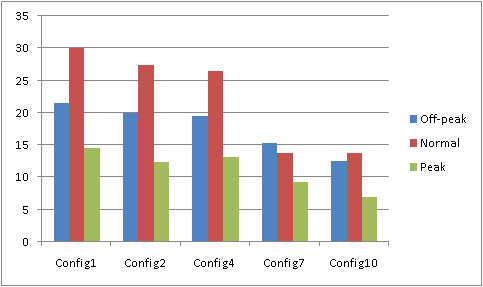
\includegraphics{Graphics/Throughput2.png}}
\caption{Throughput - requests per second}
\label{fig:4.2}
\end{figure}

We conclude from the results that the off-peak load does not burden the system and that the maximum throughput is reached after the off-peak load but before the high peak load. The system slows quickly as it nears the high load and we can assume that one or more of the system resources are under strain.

\subsection*{Average Response Times} 
Generally, as the page sizes are very small and the response is delivered in one HTTP packet, the time to last byte and the time to first byte will be equal.

\begin{figure}[h]
\centering
\scalebox{0.65}{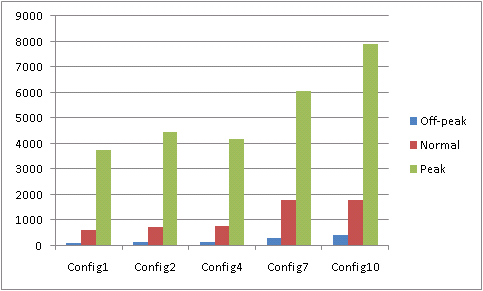
\includegraphics{Graphics/ResponseTimes2.png}}
\caption{Response Times - Time to Last Byte in Milliseconds}
\label{fig:4.3}
\end{figure}

The average response time of each of the configs for each of the loads meet the performance objective. We can see the different characteristics of each of the configs. While each of the configs shows variations in their response times on each load, there is common pattern shown in the changes to response times as the loads increase. 

\subsection*{Response Times Within 8 Seconds}
As we have a defined a maximum response time we must be careful not to just use averages in measuring the response time of the system as it does not tell us how many responses where actually outside our target. For this we measure the percentage of responses within the target.


\begin{figure}[h]
\centering
\scalebox{0.65}{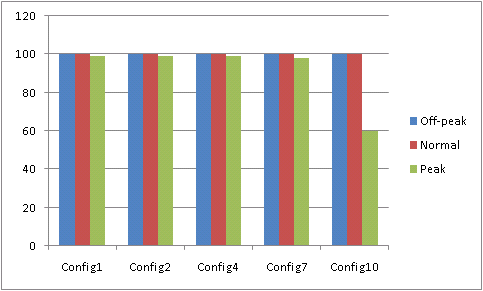
\includegraphics{Graphics/PercentWithinSLA.png}}
\caption{Percentage of responses within 8 seconds}
\label{fig:4.4}
\end{figure}

While the average response times are within the target we can see that the not all of the responses where within the target. The number of request outside the target for configs 1, 2, 4 and 7 are small however for config 10 only 60 percent of responses within 8 seconds. This is a serious problem that could stop the project from going live.


\subsection*{Errors}
Any errors returned by the server are also measured. We check the server logs for any errors that were not reported to the client. 
During the testing of the configs, on each of the different loads, no errors were recorded.



\subsection*{Resources}
We also made spot checks on the usage of server and network resources during the load test to gain a picture of the characteristics of applications. We saw that in all the tests CPU utilization was very high while memory and network usage was low. We use these measurements as inputs into our initial stress test plan. 





